% !TEX root = ../metrics_hse_exams.tex

\subsection{Demo test 1}

\begin{enumerate}
    \item We have a classical linear model 
\[
    Y_i = \beta_1 + \beta_2 X_i + u_i,
\]
where $\beta_1$ and $\beta_2$ are fixed parameters, $u_i$ is a disturbance term that is independently and identically distributed with expected value 0 and population variance $\sigma_u^2$ and $i \in \{1, \ldots, n\}$ is the observation index. 
The OLS estimation helps us to obtain the following coefficient $\beta_2$ estimator: 
\[
    \hat\beta_2 = \frac{\sum {X_iY_i}/n - \bar X \bar Y}
    {\sum {X_i^2}/n - (\bar X)^2} = 
    \frac{n \sum_{i=1}^n X_i Y_i - \sum_{i=1}^n X_i \sum_{i=1}^n Y_i}
    {n \sum_{i=1}^n X_i^2 - (\sum_{i=1}^n X_i)^2}.
\]

However, some algebraic transformations allow to show that 
\[
    \hat\beta_2 = \frac{\sum_{i=1}^n (X_i - \bar X)(Y_i - \bar Y)}
    {\sum_{i=1}^n (X_i - \bar X)^2}.
\]

Prove this is true. 

{\itshape Hint: you can try to solve backwards (going from what you are given to prove to the OLS estimator)}


\item 
A variable $Y_i$ is generated as: 
\[
    Y_i = \beta_1 + u_i,
\]
where $\beta_1$ is a fixed parameter, $u_i$ is a disturbance term that is independently and identically distributed with expected value 0 and population variance $\sigma_u^2$ and $i \in \{1, \ldots, n\}$ is the observation index. 
The least squares estimator of $\beta_1$ is $\bar Y$, the sample mean of $Y$. 
However, a researcher believes that $Y$ is a linear function of another variable $X$ and uses ordinary least squares to fit the relationship:
\[
    \hat Y_i = \hat \beta_1 + \hat \beta_2 X_i,
\]
calculating $\hat \beta_1$ as $\hat Y - \hat \beta_2 \bar X$, where $\bar X$ is the sample mean of $X$. 
Regressor $X$ may be assumed to be a nonstochastic variable. 
Determine whether the researcher’s estimator $\hat \beta_1$ is biased or unbiased, and if biased, determine the direction of the bias.


\item The output below gives the result of regressing $FDHO$, annual household expenditure on food consumed at home, on $EXP$, total annual household expenditure, both measured in dollars, using the Consumer Expenditure Survey data set. 

\begin{minipage}{\textwidth}
    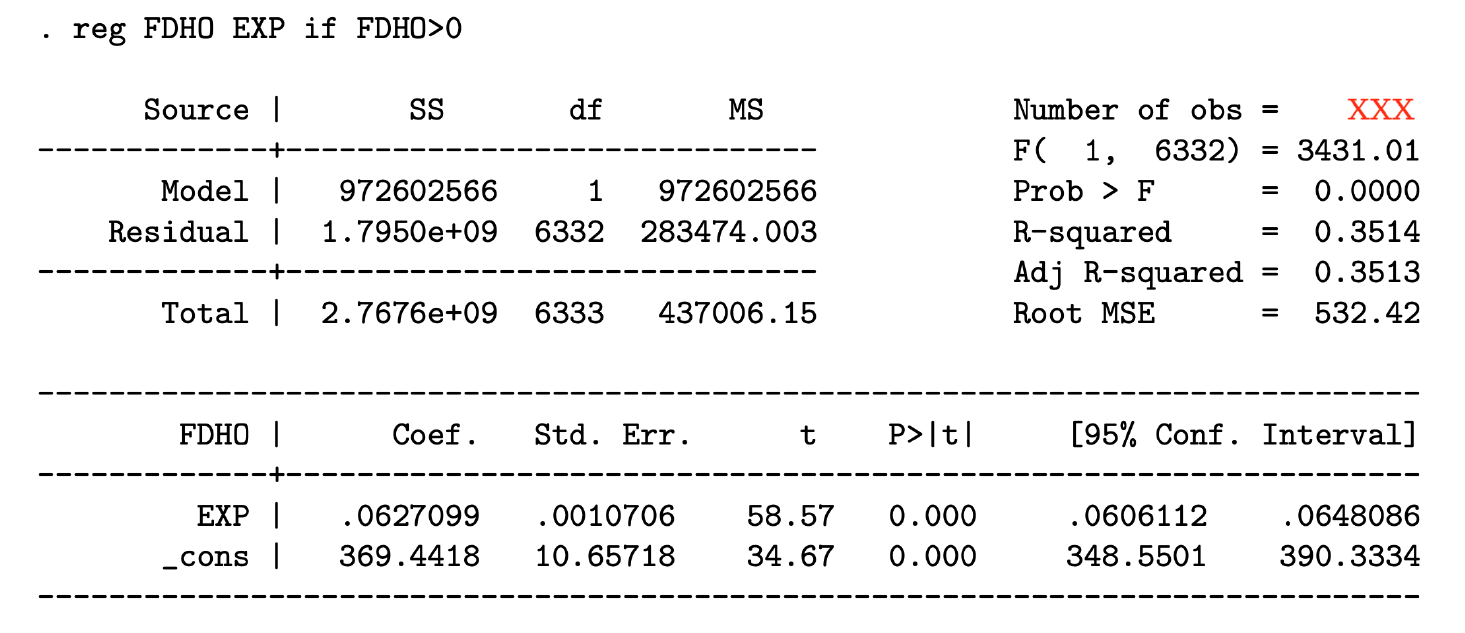
\includegraphics[width=0.85\textwidth]{figures/2021-2022_tests_stata-a.png}
\end{minipage}


Unfortunately, some things are missing. Looking at this output, do the following tasks:

\begin{enumerate}
    \item 
    Give an interpretation of the coefficients estimations.
    
    \item
    Find the number of observations.
    
    \item
    Find the values of TSS, ESS and RSS.
    
    \item
    Explain in your own words what TSS, ESS and RSS are or provide formulas for them.
\end{enumerate}


\item We have a classical linear model 
\[
    Y_i = \beta_1 + \beta_2 X_i + u_i,
\]
where $\beta_1$ and $\beta_2$ are fixed parameters, $u_i$ is a disturbance term that is independently and identically distributed with expected value 0 and population variance $\sigma_u^2$ 
and $i \in \{1, \ldots, n\}$ is the observation index.

Derive the OLS  $\hat \beta_1$ and $\hat \beta_2$ estimators. 
Answers without a solution will not be accepted. You need to provide a full solution.
\end{enumerate}



\subsection{Test 1}

You have 40 minutes to complete the test. Please explain each step of your derivations and state all the assumptions employed. 
Note that different problems can give you different points. Maximum for the test is 10 points.  

\begin{enumerate}
    \item Some practitioners of econometrics consider regressions with transformed variables. 
    For example, if the original model specification is
\[
    Y_i = \beta_1 + \beta_2 X_i + u_i,
\]
the revised specification is
\[
    Y_i^* = \beta_1^* + \beta_2^* X_i^* + v_i,
\]
where
\[
    Y_i^* = \frac{Y_i - a}{c} \text{ and } X_i^* = \frac{X_i - b}{d}.
\]

Knowing that $a, b, c, d$ are some constants and $ c \ne 0, d \ne 0$, express the OLS estimators $\hat\beta_1^*$, $\hat\beta_2^*$ 
in terms of the OLS estimators $\hat\beta_1$, $\hat\beta_2$ [2 points].


\item A novice econometrician estimated a classical linear model 
\[
     Y_i = \beta_1 + \beta_2 X_i + u_i
\]
using 4 observations and obtained the following results:

\begin{tabular}{@{}ccccc@{}}
\toprule
 $Y_i$ & 3 & 7 & 9 & 10\\ 
 $X_i$ & 3 & XXX & XXX & 1\\ 
 $\hat Y_i$ & 4 & 8 & 7 & 11\\ 
\bottomrule
\end{tabular}

Help this econometrician find the estimates of the regression coefficients $\hat \beta_1$ and $\hat \beta_2$ [1 point] and restore the missing values in table [1 point]. 
Can you confirm that these estimations were made using the OLS method? [1 point]

\item 
The output below gives the result of regressing $WAGE$, individual monthly wage measured in thousand rubles, on $TENURE$, total years of work experience a person has.

\begin{minipage}{\textwidth}
    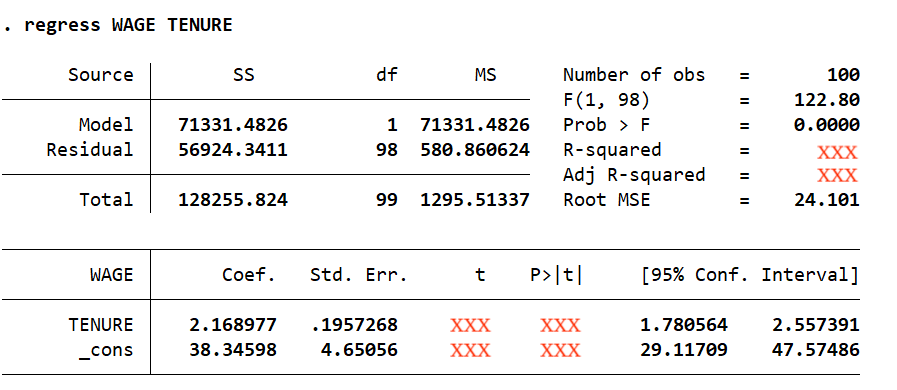
\includegraphics[width=0.85\textwidth]{figures/2021-2022_tests_stata-b.png}
\end{minipage}


Unfortunately, some things are missing. Looking at this output, do the following tasks:

\begin{enumerate}
    \item 
    Give an interpretation of the coefficients estimations [1 point].
    
    \item
    Tell whether coefficients are statistically significant or not (if necessary, you may assume that these hypotheses are tested at a $5\%$ significance level, $t_{crit} \approx 2$) [1 point].
    
    \item
    Find the $R^2$ value [0.5 points].
    
    \item
    Explain in your own words what the $R^2$ value shows [0.5 points].
    
\end{enumerate}

\item We have a linear model 
\[
    Y_i = \beta X_i + u_i,
\]
where $\beta$ is a fixed parameter, $u_i$ is a disturbance term that is independently and identically distributed with expected value 0 and population variance $\sigma_u^2$ 
and $i \in \{1, \ldots, n\}$ is the observation index.


Derive the OLS  $\hat \beta$ estimator. 
Answers without a solution will not be accepted. You need to provide a full solution [2 points].

\end{enumerate}


\subsection{Test 1, answers}

\begin{enumerate}
    \item 
\[
\hat\beta_1^* = \frac{\hat\beta_1 + b \hat\beta_2 -a}{c}, \quad \hat\beta_2^* = \frac{d\hat\beta_2}{c}
\]
\item $\hat\beta_1 = 29/2$, $\hat\beta_2 = -7/2$, $X_2 = 13/7$, $X_3 = 15/7$, 
coefficients were not estimated with OLS as $\sum \hat u_i \neq 0$.
\item 
\begin{enumerate}
    \item A one-year increase in tenure is associated with a 2.2 thousand rubles increase in wage.
    The minimal wage a novice worker (with no experience) gets is 38.5 thousand rubles.
 \item 
 \item $R^2 = 0.556$
 \item $R^2$ is interpreted as the fraction of the sample variation in the response variable that
 is explained by explanatory variables. It shows how well the data fit the regression
 model.

\begin{minipage}{\textwidth}
    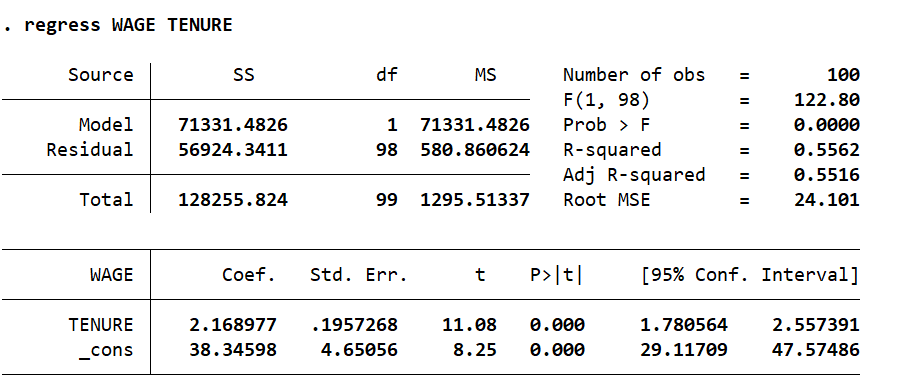
\includegraphics[width=0.85\textwidth]{figures/2021-2022_tests_stata-c.png}
\end{minipage}

\end{enumerate}
\item $\hat\beta = \sum X_i Y_i / \sum X_i^2$
\end{enumerate}

\subsection{Test 2}

You have 40 minutes to complete the test. Please explain each step of your derivations and state
all the assumptions employed. Note that different problems can give you different points.
Maximum for the test is 10 points.


\begin{enumerate}

\item An econometrician estimated this model with $N=55$ observations
\[
\hat{Y}_i = \underset{(0.3)}{3.5} + \underset{(0.4)}{6.1} A_i - \underset{(0.2)}{4.1} B_i. 
\]
Assuming the disturbance term has a standard normal distribution, calculate the 95\%
confidence interval for $\beta_1$ and $\beta_2$ [1 point].
What can you conclude from this calculation [1 point]?


\item An econometrician estimated the model with N observations (persons). In this model: $Earnings$
— hourly earnings of person (\$), $S$ — number of years of study. 
Along with the coefficient estimates, the researcher also got the $R^2$ value.
\[
\widehat{Earnings}_i = \underset{(0.3)}{3.1} + \underset{(?)}{6.1} H_i, R^2= 0.43. 
\]

\begin{enumerate}
    \item Assuming the disturbance term has a standard normal distribution, perform an $F$-test on the
    goodness of fit of the equation writing down the null and alternative hypotheses. What can you
    conclude from this calculation [1 point]?
\item  Give an interpretation of the coefficients estimates [1 point].
\end{enumerate}


\item An econometrician estimated two linear models based on the same 90 observations (persons). In
this model: $Grade$ — the grade a student got for his econometric test (points, out of 10), $H$ — hours
of studying before the test.

Model 1:
\[
\widehat{Grade}_i = \underset{(0.2)}{2.3} + \underset{(0.4)}{3.25} H_i, \quad R^2= 0.43. 
\]
Model 2:
\[
\widehat{Grade}_i = \underset{(0.3)}{4.64} H_i, \quad R^2= 0.52. 
\]
Which model would you use? Explain [2 points].


\item A researcher investigating the determinants of the demand for public transport in a certain city has
the following data for 100 residents for the previous calendar year: expenditure on public transport,
$E$, measured in dollars; number of days worked, $W$; and number of days not worked, $NW$ (by
definition, $NW$ is equal to $365 – W$). He attempts to fit the following model
\[
E_i = \beta_1 + \beta_2 W_i + \beta_3 NW_i + u_i.    
\]

\begin{enumerate}
\item Explain why it is impossible to fit this equation. Give intuitive explanations [1 point].
\item The researcher estimated model using the OLS method. What can we say about the OLS estimator
of coefficients if $u_i$ is a disturbance term that is independently and identically distributed with
expected value $a\neq 0$ [1 point].
\end{enumerate}


\item Prove that the OLS estimator of coefficients in a multiple regression is unbiased 
if the Gauss–Markov conditions are satisfied (use the matrix notation) [1 point].

Derive the variance of the coefficients (use the matrix notation) [1 point].

\end{enumerate}


\subsection{Test 3}
You have 40 minutes to complete the test. Please explain each step of your derivations and state
all the assumptions employed. Note that different problems can give you different points.
Maximum for the test is 10 points.

\begin{enumerate}
\item You are given the following data on 2,000 respondents:
\begin{itemize}
    \item  hourly earnings (Y);
    \item  educational attainment (years) (EDUC);
    \item  total expenditure in year (TE);
    \item  value of the respondent’s house (H);
    \item  mother’s and father’s educational attainment (MEDUC and FEDUC);
    \item  Weight (W);
    \item  Sex (S);
    \item whether the main job was in the government sector or the private (G).
\end{itemize}

As a policy analyst, you are asked to investigate whether there is a difference in estimated impact
of education on earnings for different genders.

Write one equation you can estimate to test this hypothesis. Explain why you chose these
variables, type of model (nonlinear or linear) [1.5 points].

Tell whether a Chow test can be used to test this hypothesis. If not, explain why. If yes, show
how you would perform this test [1 point].

\item An econometrician estimated two models with 100 observations (s.e. in brackets):
\[
\widehat{\ln Y}_i = \underset{(0.2)}{-0.5} + \underset{(0.3)}{3.1} \ln X_i + \underset{(0.1)}{0.4} W_i. 
\]
Assuming the disturbance term has a standard normal distribution, calculate the 95 per cent
confidence intervals for coefficients estimates for $\ln X_i$ and $W_i$. 
Write an interpretation of one of the intervals [1 point].
\[
    \hat{Y}_i = \underset{(0.2)}{-0.5} + \underset{(0.5)}{2.0} X_i + \underset{(3.1)}{2.4} W_i + + \underset{(3.0)}{1.3} D_i + \underset{(1.0)}{2.1} D_i X_i.     
\]
Give interpretation of the coefficients estimates for \textbf{both} models [2 points].

\item An econometrician gained some data from a university and estimated a model based on 300
observations
\[
GPA_i = \beta_1 + \beta_2 Class_i + u_i,
\]
where GPA is the average grade of a student, CLASS is the percentage of attended classes, $u_i$ is a
disturbance term.

The econometrician thinks that talent also must influence the average grade a student gets,
however, this factor is impossible to observe and measure. Thus, the researcher supposes that there
is an endogeneity problem since the effect of talent goes to the disturbance term and talent might
correlate with the percentage of attended classes.

What will happen with the coefficients estimates in case of the endogeneity problem [0.5 points]?

The researcher discovered that the university could provide him with the data on the distance from
a student's house to the university. Explain why this distance factor can be used as an instrumental
variable [1 point].

\item An econometrician estimated the following model with 100 observations:
\[
E_i = \beta_1 + \beta_2 X_i + \beta_3 Z_i + u_i.    
\]

Suspecting that the regression was subject to heteroskedasticity where $\Var(u_i \mid X_i, Z_i) = f(Z_i)$, 
the researcher prepared the following data:


\begin{tabular}{@{}cc@{}}
    \toprule
    $RSS$ from a regression based on the 50 observations with the smallest values of $Z_i$ & $200$ \\ 
    $RSS$ from a regression based on the 50 observations with the largest values of $Z_i$ & $250$ \\
    $R^2$ from auxiliary regression (squared residuals from basic regression — dependent variable 
    and $X_i$, $X^2_i$, $Z_i$, $Z^2_i$, $X_i \cdot Z_i$ — independent variables) & 0.3 \\
    \bottomrule
\end{tabular}
    
\begin{enumerate}
\item Perform the Goldfeld–Quandt test and White test and state your conclusions [2 points].
\item How do you deal with heteroskedasticity? Which methods do you know? Write at least two methods [1 point].
\end{enumerate}

\end{enumerate}

\subsection{Test 4}

You have 40 minutes to complete the test. Please explain each step of your derivations and state all the assumptions employed. 
Note that different problems can give you different points. Maximum for the test is 10 points.  

\begin{enumerate}
    \item A researcher wants to estimate the impact of students' previous achievements on their final grade for the econometrics course. He is planning to estimate the following model:
\[
    Metrics_i = \beta_0 + \beta_1 Maths_i + \beta_2 LinearAlgebra_i + \beta_3 ProbabilityTheory_i + 
    \beta_4 Statistics_i + \epsilon_i
\]
The researcher has the total of $N$ observations ($N$ students who have finished the metrics course). He assumes that:
\begin{itemize}
    \item an extra math point is twice more important than an extra statistics point;
    \item linear algebra knowledge has the same impact as probability theory knowledge.
\end{itemize}

How to test these two statements simultaneously? Which models should be estimated? Write down both models. State the null hypothesis the researcher wants to examine. Show how the F-statistics will look like indicating and explaining the numbers of degrees of freedom. [2 points]

\item The researcher wants to estimate the way person's expenditures on coffee ($COFFEE$) 
depend on his/her income ($INCOME$) and believes that it is necessary to control for a season of the year. 
The season variable ($SEASON$) has the following values: 1 for winter, 2 for spring, 3 for summer and 4 for autumn. 
The researcher assumes that a different linear relationship can correspond to each season.

Write out the equation of the model to be estimated. Indicate the meaning of all variables included in the model. [2 points]

How to test the hypothesis of a uniform (same) linear relationship between income and expenditures for all seasons? 
Carefully write out the main hypothesis, the alternative hypothesis, the formula for calculating the test statistics. [1,5 points]


\item The teacher asked you to find out which factors influence the total number of pages 
of a student's book a person reads during a week's preparation for an exam. 
You want to include the following explanatory variables:

\begin{itemize}
    \item $FREE$ — hours of free time on the week before an exam;
    \item $TRIP$ — duration of the trip from home to university (if the trip is long, a person might use this time for reading);
    \item $GRADES$ — grades for home assignments that a person received before the exam.
\end{itemize}

Your groupmate, who is doing the same task, likes the variables that you have suggested, 
but he decides to include some additional factors and his explanatory variables are:

\begin{itemize}
    \item the same factors that were suggested by you;
    \item $SEX$ — dummy on sex (females are usually more diligent and will spend more time on preparation);
    \item $BURGERS$ — the number of burgers a person has eaten during this week.
\end{itemize}

The teacher says that the first model lacks an important factor ($SEX$), while the second model has an unnecessary factor ($BURGERS$). 
All in all, both students have made some mistakes while specifying their models.
What will be the consequences of each mistake? Which mistake is more dangerous for a researcher and why? [3 points]

\item Choose one paper that was presented during the course (not the one you presented!) and write down its title or authors. 
What is the main research question of the paper? What data do authors use to answer the research question? [1,5 points]

Having studied different aspects of econometric models, 
what can you say about potential problems with the modelling that can arise here? [extra points]
\end{enumerate}
